\documentclass[journal,12pt,twocolumn]{IEEEtran}

\usepackage{setspace}
\usepackage{gensymb}
\usepackage{hyperref}
\hypersetup{
    colorlinks=true,
    linkcolor=blue,
    filecolor=magenta,      
    urlcolor=cyan,
    pdftitle={Overleaf Example},
    pdfpagemode=FullScreen,
    }

\urlstyle{same}
\singlespacing


\usepackage[cmex10]{amsmath}

\usepackage{amsthm}

\usepackage{mathrsfs}
\usepackage{txfonts}
\usepackage{stfloats}
\usepackage{bm}
\usepackage{cite}
\usepackage{cases}
\usepackage{subfig}

\usepackage{longtable}
\usepackage{multirow}

\usepackage{enumitem}
\usepackage{mathtools}
\usepackage{steinmetz}
\usepackage{tikz}
\usepackage{circuitikz}
\usepackage{verbatim}
\usepackage{tfrupee}
\usepackage[breaklinks=true]{hyperref}
\usepackage{graphicx}
\usepackage{tkz-euclide}

\usetikzlibrary{calc,math}
\usepackage{listings}
    \usepackage{color}                                            %%
    \usepackage{array}                                            %%
    \usepackage{longtable}                                        %%
    \usepackage{calc}                                             %%
    \usepackage{multirow}                                         %%
    \usepackage{hhline}                                           %%
    \usepackage{ifthen}                                           %%
    \usepackage{lscape}     
\usepackage{multicol}
\usepackage{chngcntr}

\DeclareMathOperator*{\Res}{Res}

\renewcommand\thesection{\arabic{section}}
\renewcommand\thesubsection{\thesection.\arabic{subsection}}
\renewcommand\thesubsubsection{\thesubsection.\arabic{subsubsection}}

\renewcommand\thesectiondis{\arabic{section}}
\renewcommand\thesubsectiondis{\thesectiondis.\arabic{subsection}}
\renewcommand\thesubsubsectiondis{\thesubsectiondis.\arabic{subsubsection}}


\hyphenation{op-tical net-works semi-conduc-tor}
\def\inputGnumericTable{}                                 %%

\lstset{
%language=C,
frame=single, 
breaklines=true,
columns=fullflexible
}
\begin{document}


\newtheorem{theorem}{Theorem}[section]
\newtheorem{problem}{Problem}
\newtheorem{proposition}{Proposition}[section]
\newtheorem{lemma}{Lemma}[section]
\newtheorem{corollary}[theorem]{Corollary}
\newtheorem{example}{Example}[section]
\newtheorem{definition}[problem]{Definition}

\newcommand{\BEQA}{\begin{eqnarray}}
\newcommand{\EEQA}{\end{eqnarray}}
\newcommand{\define}{\stackrel{\triangle}{=}}
\bibliographystyle{IEEEtran}
\providecommand{\mbf}{\mathbf}
\providecommand{\pr}[1]{\ensuremath{\Pr\left(#1\right)}}
\providecommand{\qfunc}[1]{\ensuremath{Q\left(#1\right)}}
\providecommand{\sbrak}[1]{\ensuremath{{}\left[#1\right]}}
\providecommand{\lsbrak}[1]{\ensuremath{{}\left[#1\right.}}
\providecommand{\rsbrak}[1]{\ensuremath{{}\left.#1\right]}}
\providecommand{\brak}[1]{\ensuremath{\left(#1\right)}}
\providecommand{\lbrak}[1]{\ensuremath{\left(#1\right.}}
\providecommand{\rbrak}[1]{\ensuremath{\left.#1\right)}}
\providecommand{\cbrak}[1]{\ensuremath{\left\{#1\right\}}}
\providecommand{\lcbrak}[1]{\ensuremath{\left\{#1\right.}}
\providecommand{\rcbrak}[1]{\ensuremath{\left.#1\right\}}}


\theoremstyle{remark}
\newtheorem{rem}{Remark}
\newcommand{\sgn}{\mathop{\mathrm{sgn}}}
\providecommand{\abs}[1]{\left\vert#1\right\vert}
\providecommand{\res}[1]{\Res\displaylimits_{#1}} 
\providecommand{\norm}[1]{\left\lVert#1\right\rVert}
%\providecommand{\norm}[1]{\lVert#1\rVert}
\providecommand{\mtx}[1]{\mathbf{#1}}
\providecommand{\mean}[1]{E\left[ #1 \right]}
\providecommand{\fourier}{\overset{\mathcal{F}}{ \rightleftharpoons}}
%\providecommand{\hilbert}{\overset{\mathcal{H}}{ \rightleftharpoons}}
\providecommand{\system}{\overset{\mathcal{H}}{ \longleftrightarrow}}
	%\newcommand{\solution}[2]{\textbf{Solution:}{#1}}
\newcommand{\solution}{\noindent \textbf{Solution: }}
\newcommand{\cosec}{\,\text{cosec}\,}
\providecommand{\dec}[2]{\ensuremath{\overset{#1}{\underset{#2}{\gtrless}}}}
\newcommand{\myvec}[1]{\ensuremath{\begin{pmatrix}#1\end{pmatrix}}}
\newcommand{\mydet}[1]{\ensuremath{\begin{vmatrix}#1\end{vmatrix}}}
\numberwithin{equation}{subsection}
\makeatletter
\@addtoreset{figure}{problem}
\makeatother
\let\StandardTheFigure\thefigure
\let\vec\mathbf
\renewcommand{\thefigure}{\theproblem}
\def\putbox#1#2#3{\makebox[0in][l]{\makebox[#1][l]{}\raisebox{\baselineskip}[0in][0in]{\raisebox{#2}[0in][0in]{#3}}}}
     \def\rightbox#1{\makebox[0in][r]{#1}}
     \def\centbox#1{\makebox[0in]{#1}}
     \def\topbox#1{\raisebox{-\baselineskip}[0in][0in]{#1}}
     \def\midbox#1{\raisebox{-0.5\baselineskip}[0in][0in]{#1}}
\vspace{3cm}
\title{Robot Navigation using Beacon Tracking}
\author{K.A. Raja Babu}
\maketitle
\newpage
\bigskip
\renewcommand{\thefigure}{\theenumi}
\renewcommand{\thetable}{\theenumi}
\tableofcontents
\section{ALGORITHM}
\subsection{\textbf{Components}}
\url{https://github.com/ka-raja-babu/Beacon-Tracking-for-Robot-Navigation/blob/main/Component%20list.pdf}
\subsection{\textbf{Wiring Diagram}}
\url{https://github.com/ka-raja-babu/Beacon-Tracking-for-Robot-Navigation/blob/main/Wiring%20Diagram.pdf}
\subsection{\textbf{Codes}}
\subsubsection{\textbf{ESP32 code}}
\begin{enumerate}
    \item Connect the ESP32 board to Laptop/PC using Type-B USB cable.
    \item Open the \href{https://github.com/ka-raja-babu/Beacon-Tracking-for-Robot-Navigation/blob/main/Codes/ESP32_Code.ino}{ESP32 Code} in Arduino IDE. 
    \item From Tools menu, select suitable "Board" and "Port" for your ESP32 board.
    \item Compile the code by clicking on "Verify" option.
    \item Upload the code to ESP32 using the "Upload" option.
\end{enumerate}
\subsubsection{\textbf{Arduino code:}}
\begin{enumerate}
    \item Connect the Arduino uno board to Laptop/PC using USB cable.
    \item Open the \href{https://github.com/ka-raja-babu/Beacon-Tracking-for-Robot-Navigation/blob/main/Codes/ESP32_Code.ino}{Arduino Code} in Arduino IDE. 
    \item From Tools menu, select Board as "Arduino Uno" and suitable "Port" on which the Arduino board is connected.
    \item Compile the code by clicking on "Verify" option.
    \item Upload the code to ESP32 using the "Upload" option.
\end{enumerate}
\subsection{\textbf{Working}}
\begin{enumerate}
    \item Initially, ESP32 mounted on the robot will read RSSI (Radio Signal Strength Indicator) levels in forward, right and left direction by suitable in-place rotation.
    \item Average of 20 RSSI values are taken while measuring RSSI level in a particular direction. This is done in order to read accurate RSSI levels.
    \item The robot then rotates towards the direction having the highest RSSI level.
    \item Further, It moves forward with a distance depending on the free space available in front of it. The free space in front of the robot is measured using ultrasonic sensor.
    \item By repeating above steps again and again, the robot navigates towards the beacon.
\end{enumerate}
\subsection{\textbf{Observaion / Conclusion}}
\begin{enumerate}
    \item This algorithm based on beacon tracking is successful in navigation of arduino based robot. This technology makes robot navigation quite easy to use as well as power efficient.
    \item However,this algorithm is not fully efficient.Frequent left and right rotations are required to identity the direction having the maximum RSSI level.
    \item Using this algorithm, only 60-70 percent of the time (i.e. 60-70\% Accuracy), the robot rotates and moves towards the correct direction. Due to low accuracy,the robot may take time to reach till the beacon. 
    \item This algorithm can be further optimized using any optimisation technique to increase accuracy level for navigation .
\end{enumerate}

\newpage
\subsection{\textbf{Images}}

\numberwithin{figure}{section}
\begin{figure}[!ht]
\centering
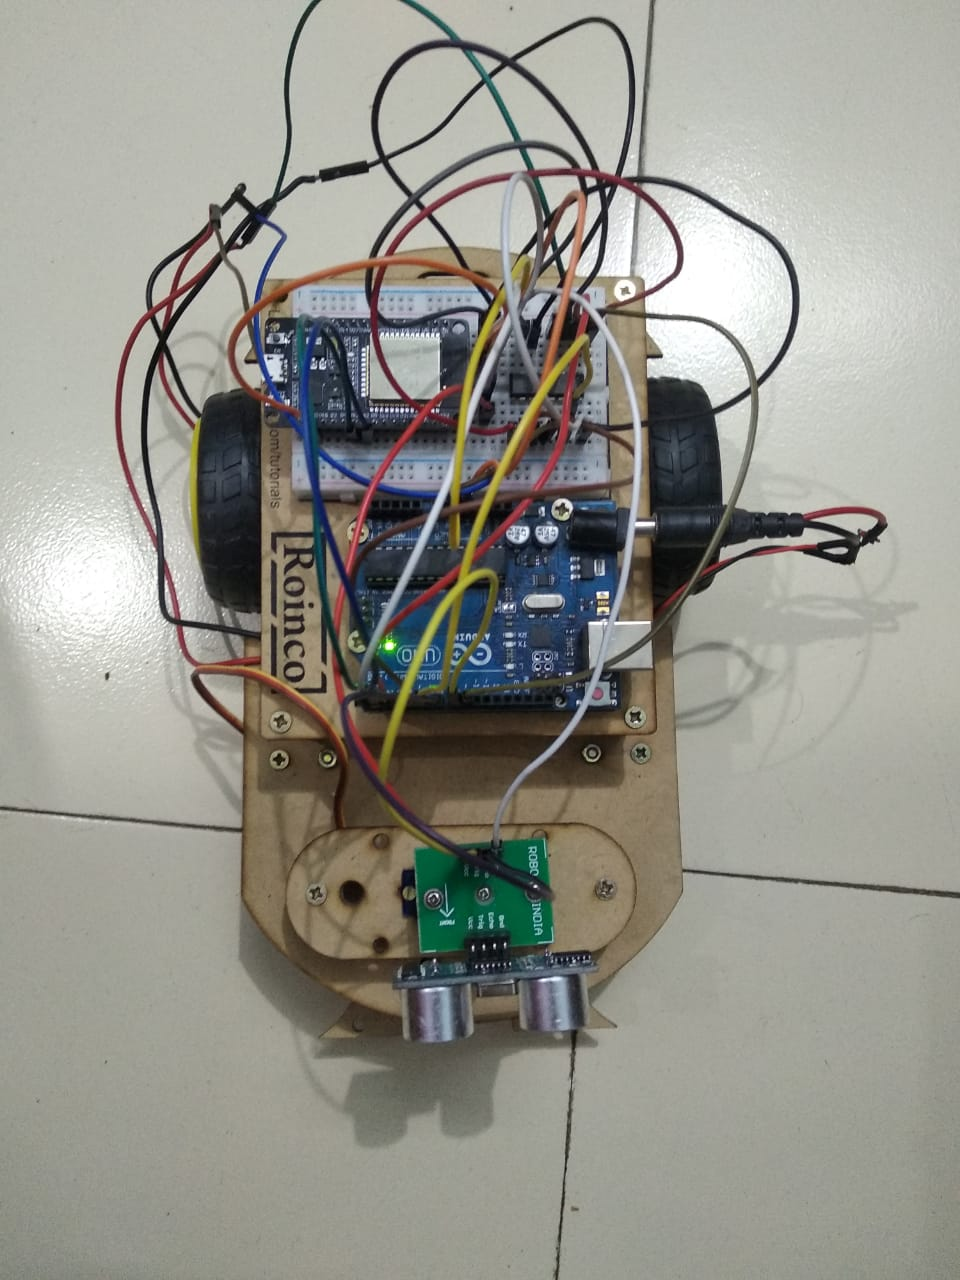
\includegraphics[width=\columnwidth]{Beacon_Tracking (1).jpeg}
\caption{Image 1}
\end{figure}

\numberwithin{figure}{section}
\begin{figure}[!ht]
\centering
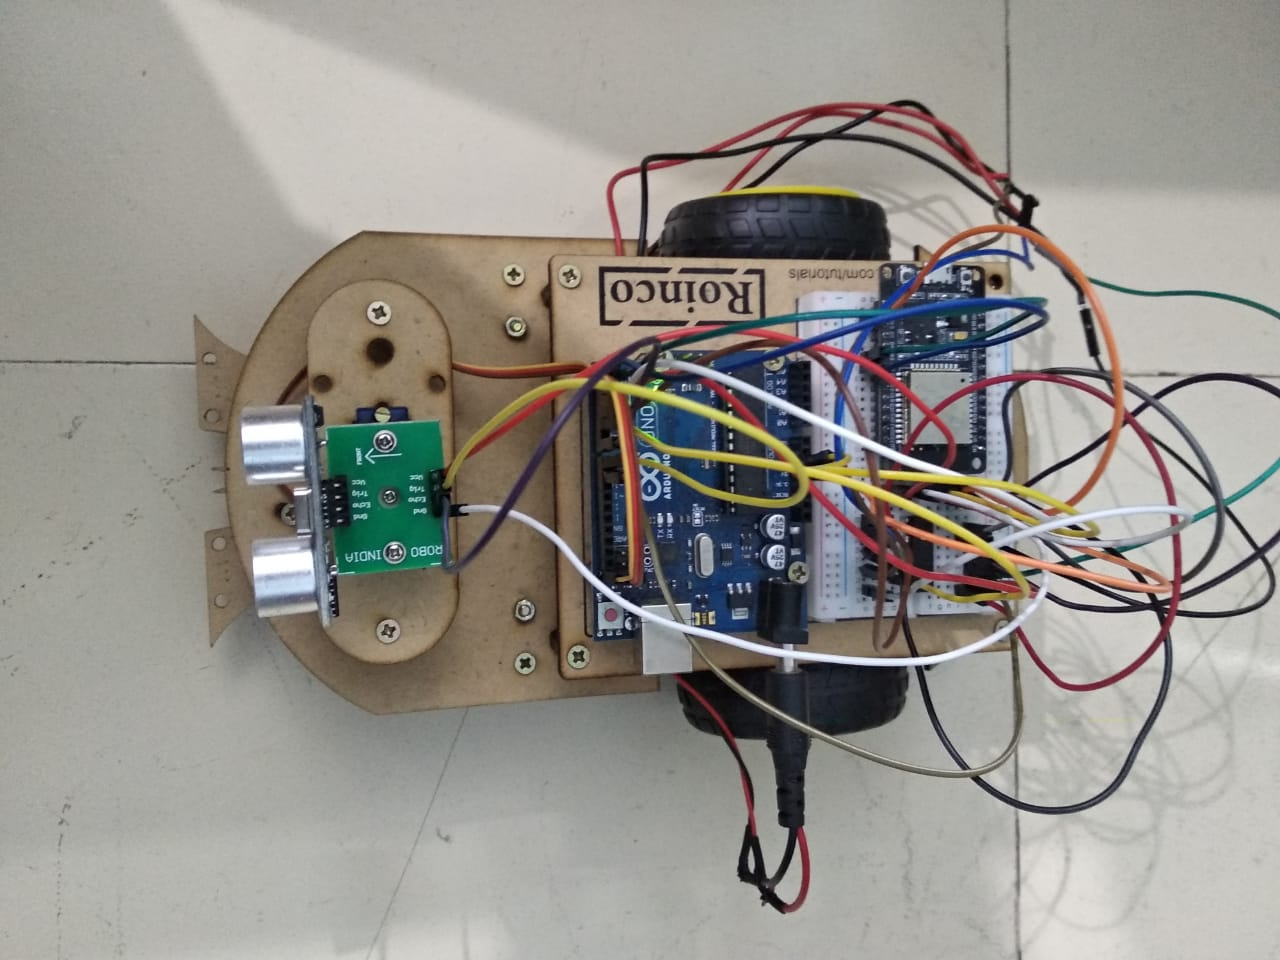
\includegraphics[width=\columnwidth]{Beacon_Tracking (2).jpeg}
\caption{Image2}
\end{figure}

\numberwithin{figure}{section}
\begin{figure}[!ht]
\centering
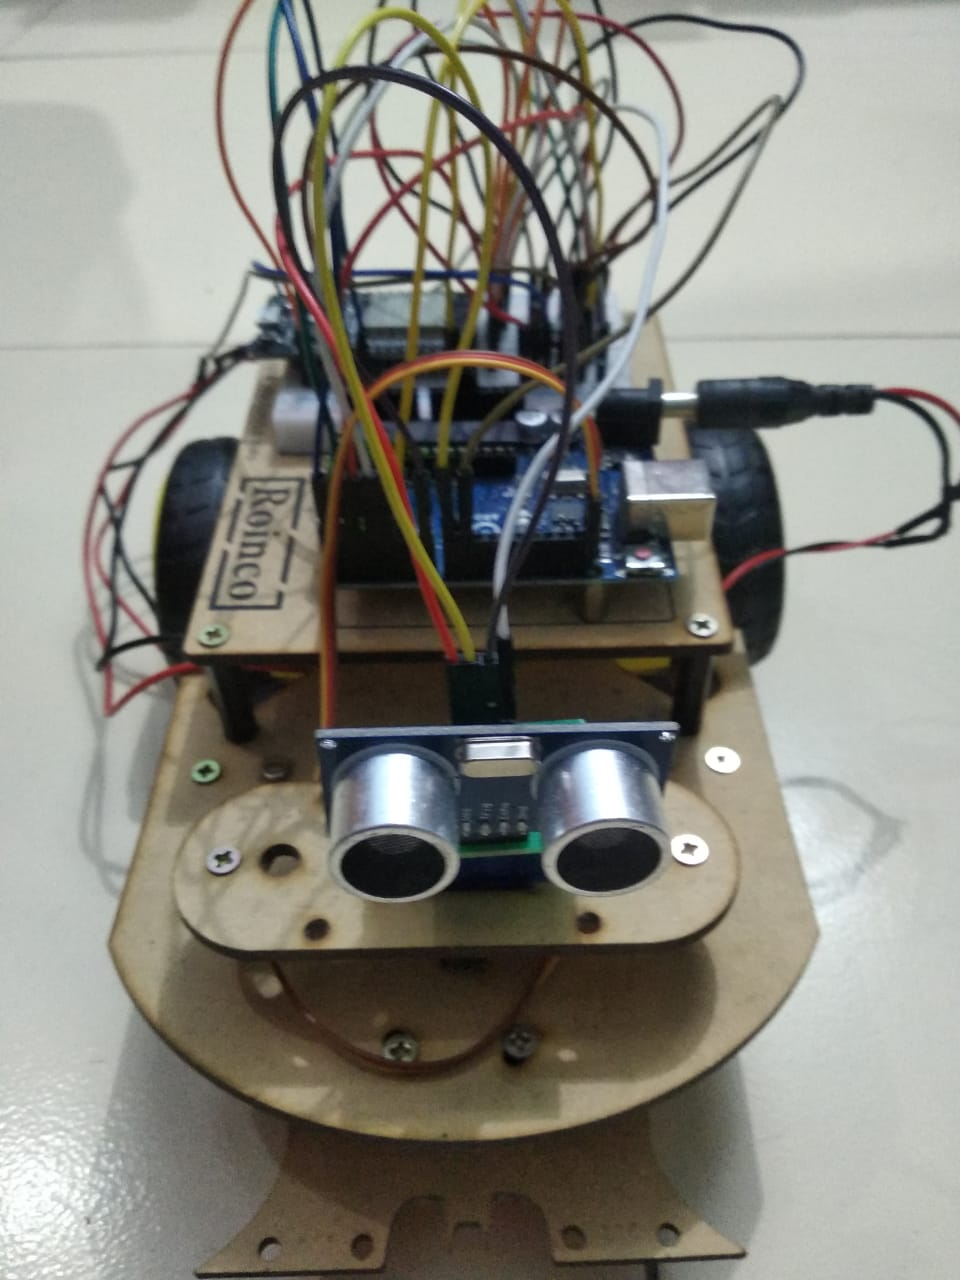
\includegraphics[width=\columnwidth]{Beacon_Tracking (3).jpeg}
\caption{Image3}
\end{figure}

\end{document}